\chapter{Entwicklung des Prototyps}
\label{ch:development}

Die Umsetzung des Prototyps erfolgt in mehreren Schritten. Zu Beginn wird wie in \ref{sub:unifiedList} beschrieben, die Liste aller Ergebnisse zusammengeführt und absteigend nach der Relevanz sortiert. Anschließend wird der Schlagwortabgleich (\ref{sub:keyword}) implementiert, indem konfigurierbar die Liste der möglichen Synonyme mit dem Suchterm abgeglichen wird und die Ergebnisse geboostet werden, wenn der Suchterm ein Synonym enthält. Zuletzt werden die resultierenden Inhalte nach einem möglichen Vorschlag wie in \ref{sub:suggestion} beschrieben dem Ergebnis hinzugefügt.

\section{Zusammengeführte Liste}
\label{sec:devUnifiedList}

Für die Entwicklung der zusammengeführten Liste im Crossload Frontend ist wichtig, dass die schon implementierte Funktionalität der Suche nach Kategorien nach der Entwicklung immer noch möglich sein muss.
Dazu finden sich auf der Suchergebnisseite mehrere Tabs, bei denen auch eine Suche innerhalb von Kategorien möglich ist.
Sie wird angeführt von der gemischten Suchergebnisseite, auf der wir momentan die Aufteilung in verschiedene Kategorien sehen (\ref{fig:crossloadSuche}).

\begin{figure}[h]
  \begin{centering}
    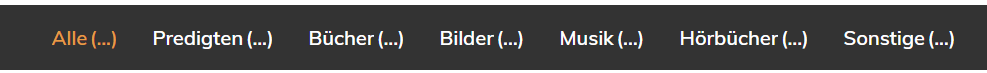
\includegraphics[width=\textwidth]{figures/development/kategorienLeiste.png}
    \caption{Leiste der Suchergebnisse in den verschiedenen Kategorien  \cite{pfleiderer2022}.}
    \label{fig:kategorienLeiste}
  \end{centering}
\end{figure}

Ziel ist es, die gemischte Suchleiste so zu ändern, dass eine große Liste mit allen Kategorien gemischt angezeigt wird.
Dazu wird die bisherige Implementation wie folgt geändert:

Anstatt nach Ergebnissen pro Kategorie abzufragen und diese in den einzelnen Sektionen darzustellen, muss eine gesammelte Anfrage an die Such API gesendet werden.
Diese wird nach dem gegebenen Sortierkriterium, in diesem Fall absteigend nach Relevanzscore sortiert von der Such API zurückgegeben.
Dafür wird zu den vorhandenen Kategorien eine „gemischte“ Kategorie hinzugefügt, bei welcher dann kein Suchfilter mitgegeben wird.
Danach sind nur noch kleine Änderungen notwendig, um das für den Nutzer schön dargestellt zu bekommen.

\begin{lstlisting}[language=Java, title={Erstellen der gemischten Kategorie \cite{frontend2022}}]
  export const MIXED_RESULTS_OPTION = {
    category: "mixed",
    path: RESULTS_BASE_URL + "/gemischt",
    lastPathSegment: "gemischt",
    text: "Alle",
    longText: "",
  } as const
\end{lstlisting}

\begin{lstlisting}[language=Java, title={Löschen der Kategorie aus den API Parametern \cite{frontend2022}}]
  if (category === "mixed") {
    delete url.category
  }
\end{lstlisting}

Das Ergebnis zeigt eine zusammengeführte Liste, die komplett nach Relevanz sortiert ist (\ref{fig:crossloadSucheNeu}).

\section{Schlagwortabgleich}
\label{sec:devKeywords}

Für den Schlagwortabgleich werden die Synonyme in Java konfiguriert.
Dazu wird eine Enumeration erstellt, die eine Liste der Synonyme enthält (\ref{annex:sourceCode}).
Durch diese Enumeration können Änderungen leicht eingebaut werden und durch die vorhandene \gls{ci}/\gls{cd} Pipeline direkt in die produktive Umgebung eingespielt werden.
Somit wäre der Nachteil der fest definierten Synonyme ausgeglichen, da Korrekturen schnell eingespielt werden können.

Eine Alternative zur Konfiguration in Java wäre eine ausgelagerte \gls{json} Datei.
Da diese aber genau wie die Java Enumeration, durch die CI/CD Pipeline, in die produktive Umgebung gelangen würde, wäre kein großer Nutzen dabei, eine JSON Datei der Enumeration vorzuziehen.
Der Unterschied dabei ist aber die Komplexität beim Einlesen der Datei und die fehlende Typisierung in der JSON Datei.
Aus diesem Grund wurde sich für die Enumeration entschieden.

Der nächste Schritt ist der Vergleich des Suchterms mit den verfügbaren Synonymen.
Dazu wird überprüft, ob dieser ein Synonym komplett enthält.
Damit sind auch Sonderfälle wie der Plural oder Beugungen enthalten, da für mögliche Spezialfälle bereits Synonyme in die Listen eingefügt wurden.

Für die Überprüfung werden Java Streams benutzt.
Diese machen den Source Code lesbarer und kleiner, da viele Kontrollstrukturen wegfallen.
Mithilfe der vorhandenen Klasse CrossloadCriteriaBuilder werden alle Inhalte der gefundenen Kategorie geboostet.
Für Predigten wird hierbei noch für den Spezialfall der Predigt mit Video unterschieden, bei nur Predigten mit Video geboostet werden und andere Predigten keine besondere Behandlung erfahren.

\begin{lstlisting}[language=Java, title={Code für Überprüfung und Boosten der Kategorien. \cite{solr-search2022}}]
  private void addCategoryBoost(String searchTerm, SolrQuery query) {
    SermonCategory.getAllCategories()
      .stream()
      .filter(category -> category.hasCategory(searchTerm))
      .forEach(category ->  {
        CrossloadCriteriaBuilder instance = CrossloadCriteriaBuilder.getInstance();
        // Boost für Inhalte mit Videos, falls ein Videosynonym gefunden.
        if(SermonCategory.VIDEO.equals(category)) {
          instance.addCriteria(SchemaField.HAS_PRIMARY_VIDEO, "true", 75);
          query.addCriteria(instance);
        }
        else {
          // Boosten der gefundenen Kategorie
          instance.addCriteria(SchemaField.MAIN_CAT, category.getId(), 3);
          query.addCriteria(instance);
        }
      });
  }
\end{lstlisting}

\section{Vorschläge für weitere Navigation}
\label{sec:devSuggestions}

% TODO Adjust Schema, -> add suggestion object
% TODO Create Function to determine suggestion
% TODO Add Suggestion to result
